\documentclass{siproblemset}


% SI Session Information
\course{MTH 1321}       % the course of your SI
\sessionnum{idk}         % (optional) specify the session number
\sessiondate{11/29/21}   % the date of the session

\warmup{Concept Review}
\topic{FTOC 1}
\topic{FTOC 2}
%\cooldown{Review}

% Worksheet Information
\title{The Fundamental\linebreak Theorem of Calculus}
\sections{Section 5.4-5.5}
\withnamespace

\begin{document}
    \maketitle
    
    \activity{Warmup}{Concept Review}{Work \textbf{alone} to answer these questions. Try not to use your notes.}{10 minutes}
 
    \frq{What is the Fundamental Theorem of Calculus, Part I?}
    \Smallsp
    
    \frq{What is the Fundamental Theorem of Calculus, Part II?}
    \Smallsp
    
    \frq{What is the area/accumulation function?}
    \smallsp
    
    \frq{How do you find the \textbf{total} area between a curve and the $x$-axis?}
    \smallsp

    \newpage
    
    \activity{Activity 1}{Definite Integrals}{Make a \textbf{group of two or three, all with the same colored worksheets}, to work together to do your assigned parts. Then, try to do the other parts. Try not to use your notes. \textbf{DO NOT use a calculator}.}{30 minutes}
    
    \mcq{Compute the following definite integrals.}{
%        \task $\int_{-2}^{-1}\dfrac{1}{x^3}\text{d}x$
%        \normalsp
%        \task $\int_{-1}^1(5u^4+u^2-u)\text{d}u$
%        \normalsp
        \task $\int_1^{27}\dfrac{t+1}{\sqrt{t}}\text{d}t$
        \normalsp
        \task $\int_0^{13\pi}(2\sin(x)-3\cos(x))\text{d}x$
        \normalsp
%        \task $\int_2^6\left(x+\dfrac{1}{x}\right)\text{d}x$
%        \normalsp
        \task $\int_{\pi/6}^0\sec(\theta)\tan(\theta)\text{d}\theta$
        \normalsp
    }
    
    \newpage
    \frq{Use FTOCI to find the explicit formula for the area function represented by the following integral.}
    $$\int_{4}^{x}e^{3u}\dd u$$ 
    \smallsp
    
    \activity{Activity 2}{Fundamental Theorem of Calculus, Part II}{Make a \textbf{group of two or three, all with the same colored worksheets}, to work together to answer these questions. Try not to use your notes. \textbf{DO NOT use a calculator}.}{30 minutes}
   
    \mcq{Compute the following derivatives.}{
        \task $\dddf s\int_{100}^{s}\ln(6u-5)\dd u$
        \Normalsp
        \task $\dddf x\int_{2}^{x}\sin(5t)\dd t$
        \Normalsp
        \task $\dddf x\int_{0}^{x^2}\frac{t\dd t}{t+1}$
        \Normalsp
        \task $\dddf t\int_{-4}^{\sec(t)}u^3\dd u$
        \Normalsp
    }
    
    \newpage
    \activity{Activity 3}{FTOCII and Graphs}{Make a \textbf{group of two or three, all with the differently-colored worksheets}, to work together to answer these questions. Try not to use your notes. \textbf{DO NOT use a calculator}.}{30 minutes}
    
    \begin{multipartquestion}
        Let $B(x)=\int_2^xg(t)\text{d}t$. Use the graph of $g(x)$ below to compute the following quantities.
        \makebox[\width][c]{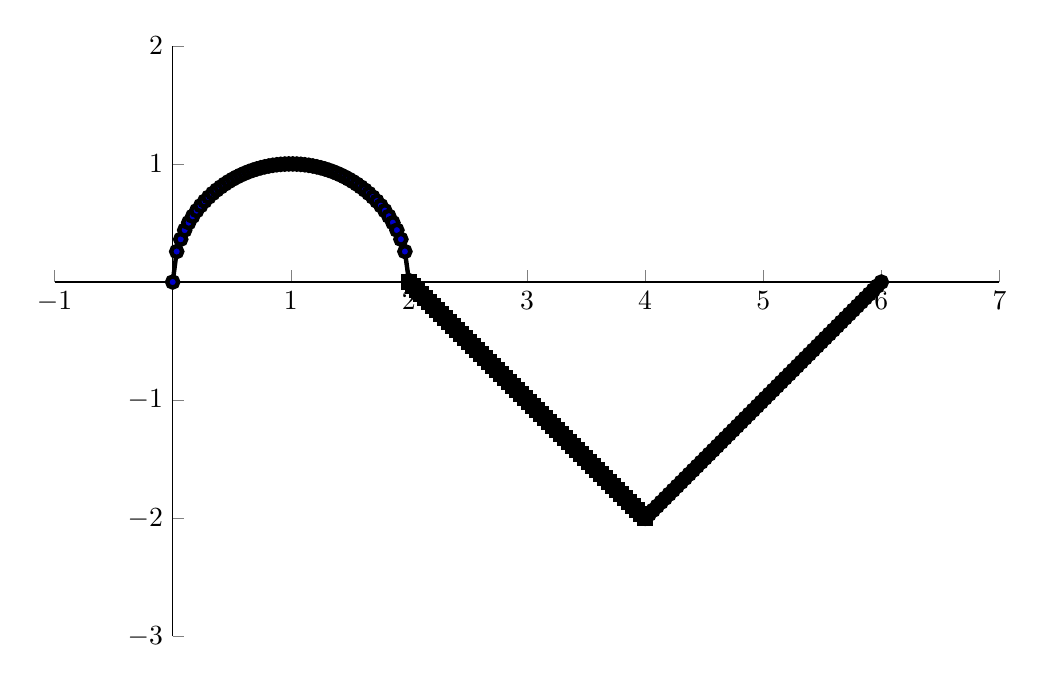
\begin{tikzpicture}[baseline=(current bounding box.north)]
            \begin{axis}[
            x=1.5cm,
            y=1.5cm,
            xmin=-1,
            xmax=7,
            ymin=-3,
            ymax=2,
            axis x line*=middle,
            axis y line*=middle,
            every axis plot/.append style={ultra thick},
            samples=60
            ]
            \addplot+[black, domain=0:2] {sqrt(1-(x-1)^2)};
            \addplot+[black, domain=2:4] {-x+2};
            \addplot+[black, domain=4:6] {x-6};
            \end{axis}
            \end{tikzpicture}}
        \frq{$B(0)$}
        \tinysp
        \frq{$B(2)$}
        \tinysp
        \frq{$B(6)$}
        \tinysp
        \frq{$B'(5)$}
        \smallsp
        \frq{$[B(5)]'$}
        \smallsp
    \end{multipartquestion}
    \newpage
    
    \begin{multipartquestion}
        Let $A(x)=\int_0^xf(t)\text{d}t$. Use the graph of $f(x)$ below to answer the following questions. 
        \makebox[\width][c]{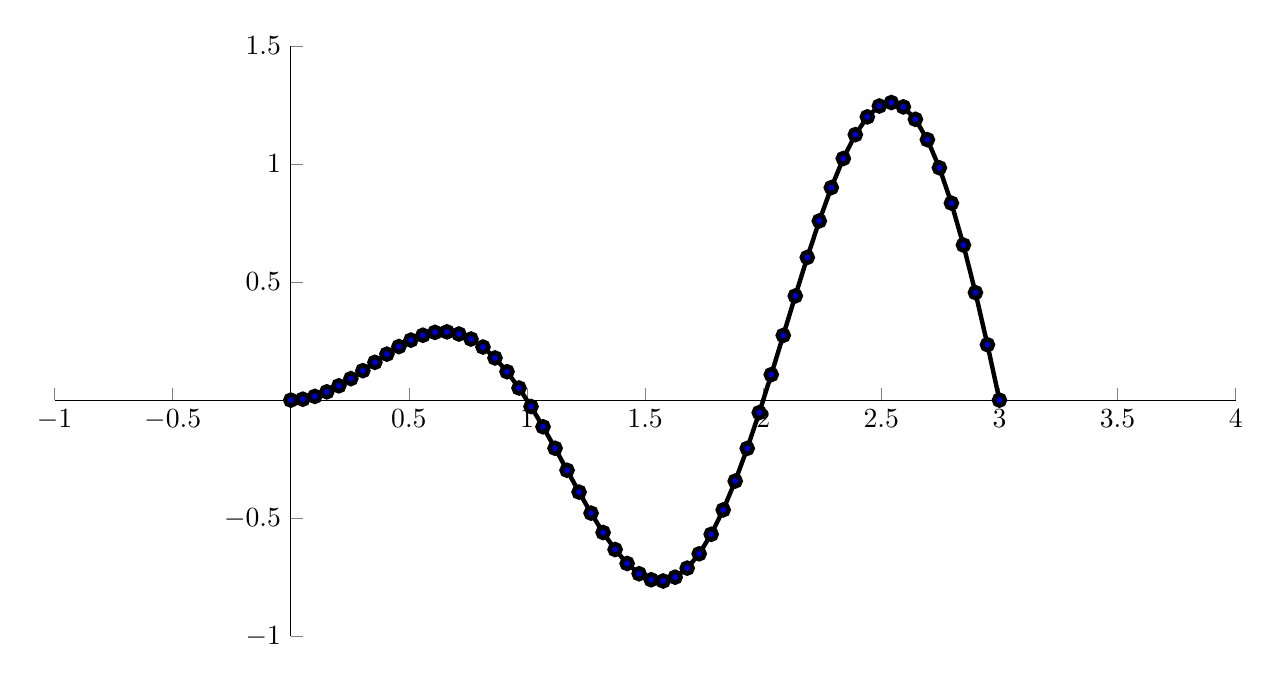
\begin{tikzpicture}[baseline=(current bounding box.north)]
            \begin{axis}[
            x=3cm,
            y=3cm,
            xmin=-1,
            xmax=4,
            ymin=-1,
            ymax=1.5,
            axis x line*=middle,
            axis y line*=middle,
            every axis plot/.append style={ultra thick},
            samples=60
            ]
            \addplot+[black, domain=0:3] {sin(180*x)*x/2};
            \end{axis}
            \end{tikzpicture}} 
        
        \frq{What are the intervals of increase and decrease for $A$?}
        \smallsp
        \frq{What are the $x$-values where $A$ has a local extremum?}
        \smallsp
        \frq{Where is $A$ concave up and down?}
        \smallsp
    \end{multipartquestion}
    
    \newpage
%
%    \activity{Cooldown}{Total Area}{Work \textbf{alone} to answer these questions. Try not to use your notes.}{15 minutes}
%        
%    \frq{Find the \textbf{total} area between the graph of $f(x)=x^2-1$ and the $x$-axis, only considering the region satisfying $-3\leq x\leq 3$.}
\end{document}